\section{Grundlagen}\label{sec:02_02_grundlagen}

\subsection{Zeittafel}\label{subsec:zeittafel}

\begin{table}[ht]
\caption{Zeittafel über die Entwicklung der europäische Union}
\label{tab:zeittafelEU}
\centering
\begin{tabular}{m{10em}|m{6em}|m{5em}|m{8em}}
\hline
\rowcolor{EUBlue}
Phase &Unterzeich- nung &In Kraft &Vertrag\\
\hline
\hline
\rowcolor{Gray}
& 1948 & 1948 & Brüsseler Pakt\\
\cline{2-4}
\rowcolor{Gray}
\multirow{-2}{*}{Westunion (WU)}& 1951 & 1952 & Paris\\
\hline
\hline
\rowcolor{Gray}
& 1954 & 1955 & Pariser Verträge\\
\cline{2-4}
\rowcolor{Gray}
\multirow{-2}{*}{Westeuro Union (WEU)}& 1957 & 1958 & Rom\\
\hline
\hline
\rowcolor{Gray}
& 1965 & 1967 & Fusionsvertrag\\
\cline{2-4}
\rowcolor{Gray}
& 1986 & 1987 & Einheitliche europäische Akte\\
\cline{2-4}
\rowcolor{Gray}
\cline{2-4}
\rowcolor{Gray}
& 1997 & 1999 & Amsterdam\\
\cline{2-4}
\rowcolor{Gray}
\multirow{-5}{*}{Euro Gemeinschafte}& 2001 & 2003 & Nizza\\
\hline
\hline
\rowcolor{Gray}
Europäische Union (EU)& 2007 & 2009 & Lissabon\\
\hline
\end{tabular}
\end{table}
\noindent
Die Entwicklung der europäische Union ist in der Tabelle~\ref{tab:zeittafelEU} zusammengefasst. 

\subsection{Montanunion (1951)}\label{subsec:montanunion}

\noindent
\begin{wrapfigure}{r}{0.3\textwidth}
  \begin{center}
    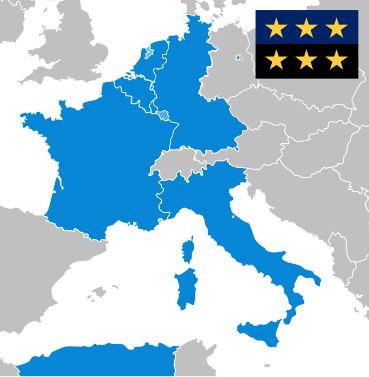
\includegraphics[width=0.3\textwidth]{images/EU_1951.png}
  \end{center}
  \caption{Die Gründungsstaaten der EU}
      \textbf{Quelle: }  \cite{montanunion1951}
  \label{fig:EU1951}
\end{wrapfigure}
\noindent
Jean Monnet schlug vor, die gesamte französisch-deutsche Kohle- und Stahlproduktion einer gemeinsamen Behörde zu unterstellen. Diese Idee wurde dann vom französischen Außenminister Robert Schuman am 9. Mai 1950 dem Parlament präsentiert, weswegen sie als Schuman-Plan in die Geschichte einging~\cite{gehlerMichaelEU}. Dieser Schuman-Plan führte am 18. April 1951 zur Gründung der Europäischen Gemeinschaft für Kohle und Stahl (EGKS, umgangssprachlich auch „Montanunion“) durch Belgien, die Bundesrepublik Deutschland, Frankreich, Italien, Luxemburg und die Niederlande~\cite{euroArchive1951}. Die Institutionen dieser EGKS bildeten den Kern der späteren EU: eine Hohe Behörde mit supranationalen Kompetenzen (aus der später die Europäische Kommission wurde), ein Ministerrat als Legislative (heute Rat der EU) und eine Beratende Versammlung (das spätere Europäische Parlament). 

\subsection{Römische Verträge (1957)}\label{subsec:roemischeVertraege}

Am 25. März 1957 bildeten die sogenannten Römischen Verträge den nächsten Integrationsschritt. Mit diesen Verträgen gründeten dieselben sechs Staaten die Europäische Wirtschaftsgemeinschaft (EWG) sowie die Europäische Atomgemeinschaft (EAG und Euratom)\cite{euroKommision1957}. Ziel der EWG war die Schaffung eines gemeinsamen Marktes, in dem sich Waren, Dienstleistungen, Kapital und Arbeitskräfte frei bewegen konnten. Durch die Euratom sollte eine gemeinsame Entwicklung zur friedlichen Nutzung der Atomenergie stattfinden. \newline
Die EU entwickelte sich dann in dem Zeitraum von 1957 bis 1990 wie auf der Abbildung~\ref{fig:eu1957Bis1990} dargestellt. 

\begin{figure}[H]
    \centering
    \subfigure[1957]
    {
        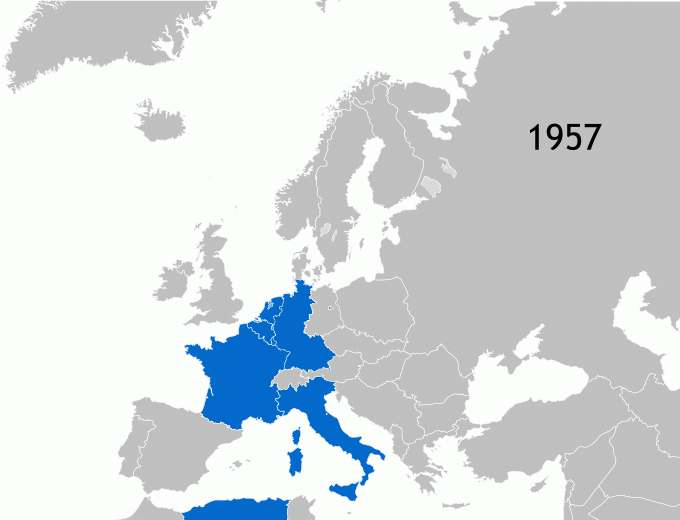
\includegraphics[width=1.65in]{images/1957.png}
        \label{fig:eu1957}
    }
    \subfigure[1973]
    {
        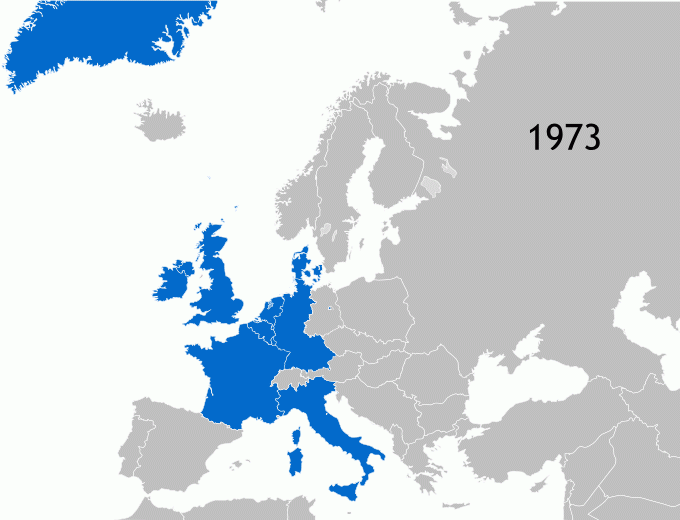
\includegraphics[width=1.65in]{images/1973.png}
        \label{fig:eu1973}
    }
    \subfigure[1981]
    {
        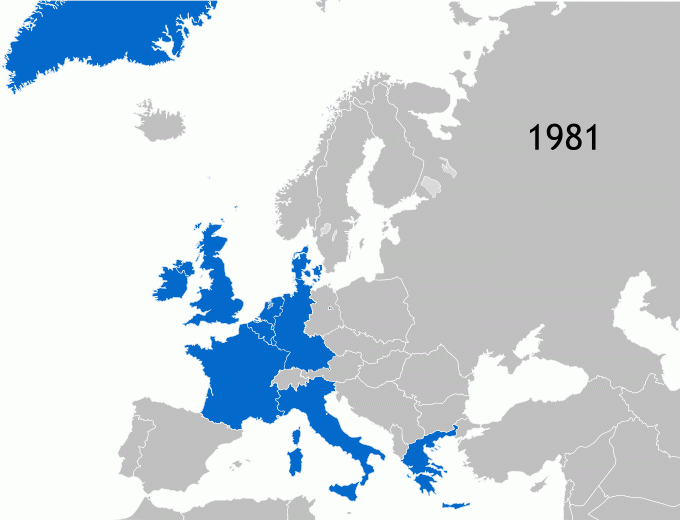
\includegraphics[width=1.65in]{images/1981.png}
        \label{fig:eu1981}
    }
    \subfigure[1986]
    {
        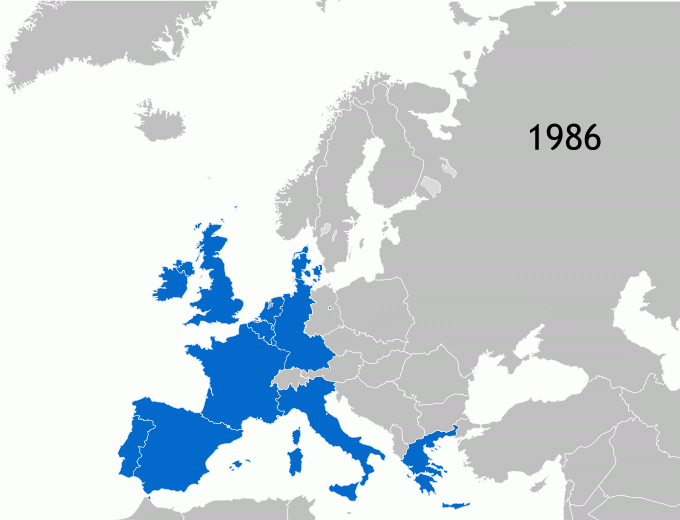
\includegraphics[width=1.65in]{images/1986.png}
        \label{fig:eu1986}
    }
    \subfigure[1990]
    {
        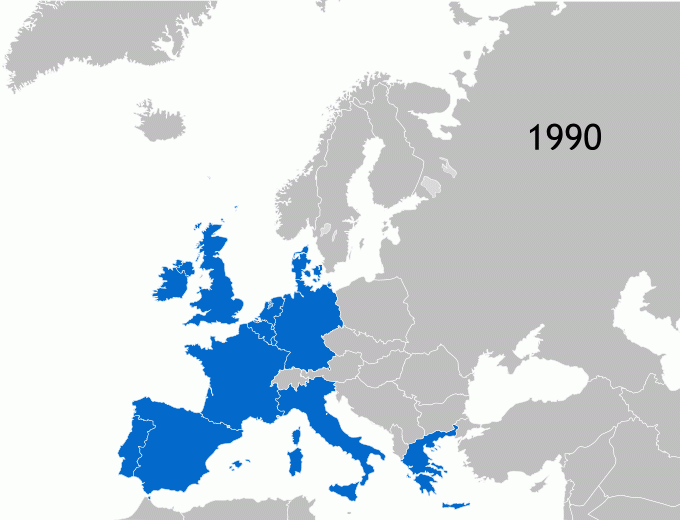
\includegraphics[width=1.65in]{images/1990.png}
        \label{fig:eu1990}
    }
    \caption{Entwicklung der EU im Zeitraum von 1957 bis 1990}
    \label{fig:eu1957Bis1990}
\end{figure}

\subsection{Vertrag von Maastricht (1992)}\label{subsec:maastricht}

Als Vertrag von Maastricht wird der Vertrag über die Europäische Union (EUV) bezeichnet, der am 7. Februar 1992 im niederländischen Maastricht vom Europäischen Rat unterzeichnet wurde. Er stellt den bis dahin größten Schritt der europäischen Integration seit der Gründung der Europäischen Gemeinschaften (EG) dar.\newline
Mit diesem Vertragswerk, das an die Stelle der 1957 geschlossenen Römischen Verträge trat, wurde die Europäische Union (EU) als übergeordneter Verbund für die Europäischen Gemeinschaften, die gemeinsame Außen- und Sicherheitspolitik sowie die Zusammenarbeit in den Bereichen Justiz und Inneres gegründet.  \newline
Abgesehen von dem eigentlichen EU-Vertrag in seiner ursprünglichen Fassung enthält der Vertrag von Maastricht auch Bestimmungen zu umfassenden Änderungen der Verträge zur Gründung der Europäischen Gemeinschaften, also des EG-Vertrags, des EURATOM-Vertrags und des damals noch in Kraft befindlichen EGKS-Vertrags. Er trat am 1. November 1993 in Kraft. Der damit geschaffene Rechtsstand wurde zum 1. Mai 1999 durch den Vertrag von Amsterdam erneut geändert. \newline
Die EU entwickelte sich dann in dem Zeitraum von 1957 bis 1990 wie auf der Abbildung~\ref{fig:eu1992Bis2004} dargestellt. 

\begin{figure}[H]
    \centering
    \subfigure[]
    {
        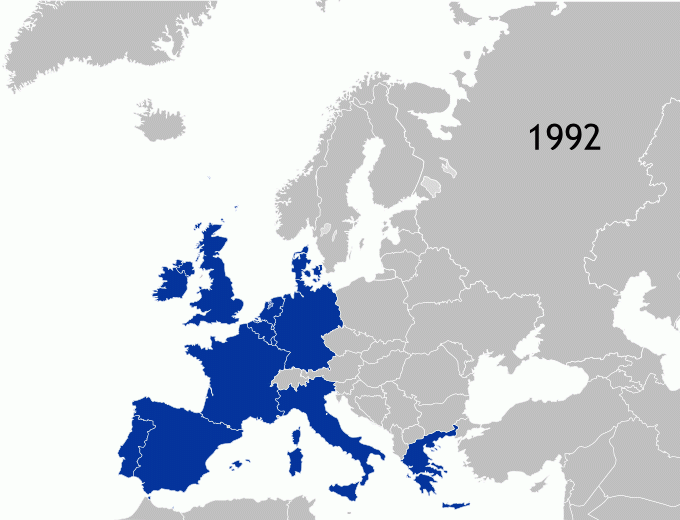
\includegraphics[width=1.65in]{images/1992.png}
        \label{fig:eu1992}
    }
    \subfigure[]
    {
        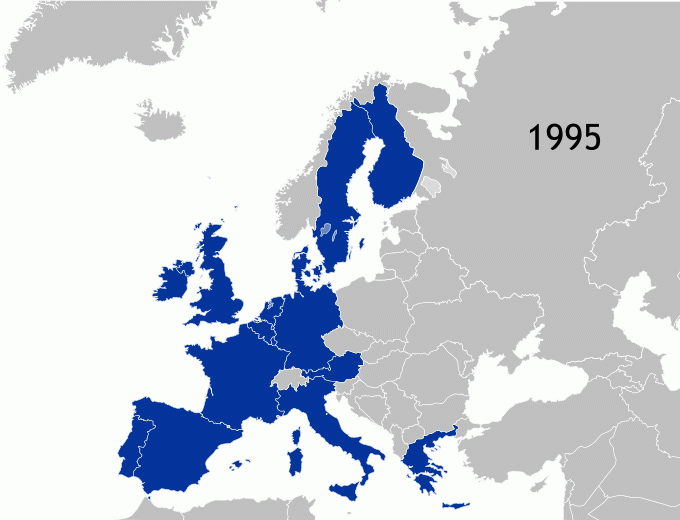
\includegraphics[width=1.65in]{images/1995.png}
        \label{fig:eu1995}
    }
    \subfigure[]
    {
        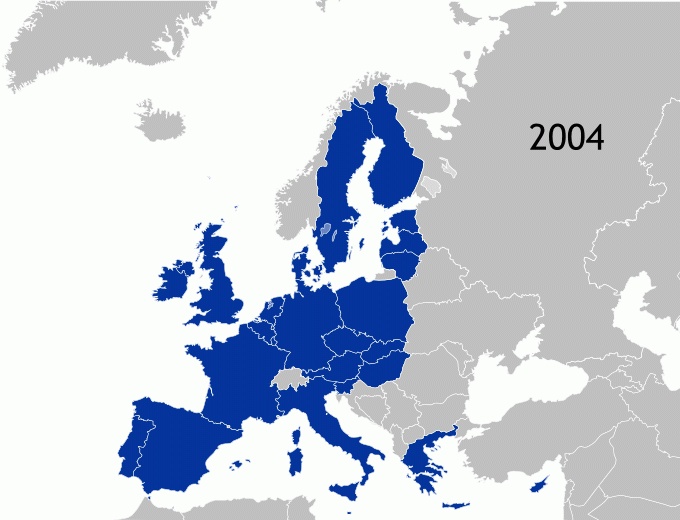
\includegraphics[width=1.65in]{images/2004.png}
        \label{fig:eu2004}
    }
    \caption{Entwicklung der EU im Zeitraum von 1992 bis 2004: 1992~\ref{fig:eu1992}, 1995~\ref{fig:eu1995}, 2004~\ref{fig:eu2004}}
    \label{fig:eu1992Bis2004}
\end{figure}

\subsection{Vertrag von Lissabon (2007)}\label{subsec:lissabon}

Der Vertrag von Lissabon (ursprünglich auch EU-Grundlagenvertrag bzw. -Reformvertrag genannt, portugiesisch Tratado de Lisboa) ist ein völkerrechtlicher Vertrag zwischen den damals 27 Mitgliedstaaten der Europäischen Union.\newline
Der Vertrag von Lissabon wurde am 13. Dezember 2007 unter portugiesischer Ratspräsidentschaft in Lissabon unterzeichnet und trat am 1. Dezember 2009 in Kraft.\newline
Der Vertrag von Lissabon reformierte den Vertrag über die Europäische Union (EU-Vertrag) und den Vertrag zur Gründung der Europäischen Gemeinschaft (EG-Vertrag), der den neuen Namen Vertrag über die Arbeitsweise der Europäischen Union (AEU-Vertrag) erhielt; ferner wurde durch Protokoll Nr.2 der Euratom-Vertrag abgeändert (siehe Art. 4 Abs. 2). 

\subsection{Phase der Herausforderungen der Union}\label{subsec:phaseHeraus}

Seit der in teilweise hohen Staatsschuldenständen resultierenden Finanzkrise ab 2007 und der daraus resultierenden Eurokrise ist die Europäische Union bei einigen ihrer Mitglieder in wirtschaftliche und soziale Turbulenzen geraten, die das Verhältnis der auf Finanzhilfen angewiesenen Mitgliedstaaten zu den für Stützungsmaßnahmen in Frage kommenden teilweise belasten. Nach 2010 wurde zur Bewältigung der Eurokrise eine Reihe von Maßnahmen eingeleitet, darunter der im Jahr 2012 eingerichtete Europäische Stabilitätsmechanismus (ESM) als Teil des Euro-Rettungsschirms sowie der Europäische Fiskalpakt, der den teilnehmenden Mitgliedsstaaten Haushaltsdisziplin und Schuldenbegrenzung auferlegt. Die Europäische Bankenunion hat ab 2014 nationale Kompetenzen auf zentrale Institutionen übertragen und damit einheitliche, gemeinsame Richtlinien und Regelungen im Bereich der Finanzmarktaufsicht und der Sanierung oder Abwicklung von Kreditinstituten innerhalb der Europäischen Union geschaffen. Auch durch das sich verstärkende und anhaltende Wirtschaftswachstum inzwischen aller Mitgliedsstaaten nach 2016 hat die Europäische Union begonnen diese Krise langsam zu bezwingen~\cite{euroKrise}. Weitere institutionelle Reformen wie eine koordinierte Wirtschafts- und Sozialpolitik oder die Weiterentwicklung des ESM zu einem Europäischen Währungsfonds stehen auf der Agenda der EU, um so zukünftige Krisen besser und schneller zu bewältigen oder sie erst gar nicht erst entstehen zu lassen.
\newline
Uneinigkeit und weitere krisenhafte Entwicklungen in der Europäischen Union hatte die Flüchtlingskrise ab 2015 zur Folge. In diesem Gesamtzusammenhang erhielten antieuropäische politische Strömungen weiteren Auftrieb. Die Flüchtlingskrise wird auch für den Austritt des Vereinigten Königreichs aus der Europäischen Union als mitursächlich angesehen. Die Aufnahmebereitschaft für Flüchtlinge bei den verschiedenen Regierungen der Mitgliedstaaten war sehr unterschiedlich und stand einem gemeinsamen Handeln der Unionsmitglieder zur Überwindung der für die gesamte Union gut bewältigbaren Krise im Wege. Teilweise kam es zur Wiedereinführung von Grenzkontrollen im Schengen-Raum; andererseits wurden diverse Vorkehrungen zum Schutz der EU-Außengrenzen getroffen, so u. a. der Ausbau von Frontex. Ein Plan zur Verteilung von Flüchtlingen unter den Mitgliedsstaaten wurde nur ansatzweise umgesetzt und durch nationalkonservative Regierungen teils offen entgegen vom EuGH höchstrichterlich bestätigter Mehrheitsentscheidungen boykottiert. Nicht nur in diesem Zusammenhang muss sich die Europäische Union bald entscheiden, mit welchen Mitteln sie künftig auf offenen Vertragsbruch dieser Regierungen reagieren soll, denn der Vertrag über die Europäische Union verpflichtet die Mitgliedstaaten der Europäischen Union zu Solidarität und Rechtsstaatlichkeit.\newline
Als eine vorrangige Herausforderung für das politische Handeln gelten den 2019 neugewählten Organen der EU die globale Erwärmung und die Herbeiführung eines wirksamen Klimaschutzes. Anlässlich der Bestätigung der neu zusammengesetzten EU-Kommission durch das Europäische Parlament gab die designierte Präsidentin Ursula von der Leyen im Rahmen eines „europäischen grünen Deals“ das Ziel aus, den Treibhausgasausstoß in der EU bis 2030 nicht wie bislang geplant um 40 Prozent zu senken, sondern um 50 Prozent. Europa solle der erste klimaneutrale Kontinent werden~\cite{tagesSpiegelEUKrise}. Am darauffolgenden Tag, dem 28. November 2019, rief das Europäisches Parlament den Klimanotstand für Europa aus. In der Konsequenz soll die Europäische Kommission ihre gesamte Politik an dem globalen Ziel ausrichten, die Erhitzung der Erde auf 1,5 Grad gegenüber vorindustriellen Zeiten zu begrenzen.